\section*{Systemtheorie der Sinnesorgane}
\setcounter{subsection}{2} 
\subsection{Übung}
\subsubsection{}
First, the reaction of an inner hair cell (IHC) to an external actuation of the stereocilia was measured for two frequencies: \SI{100}{\hertz} (Fig. \ref{fig:signal100}) and \SI{10}{\kilo\hertz} (Fig. \ref{fig:signal10k}) with \SI{100}{\nano\meter} peak displacement. We observe a saturation at the higher frequency, where the IHC cannot follow the actuation because of capacitive effects. Regarding the envelope, this cell fires one single continuous signal. 
\begin{figure}[h] 
  \centering
  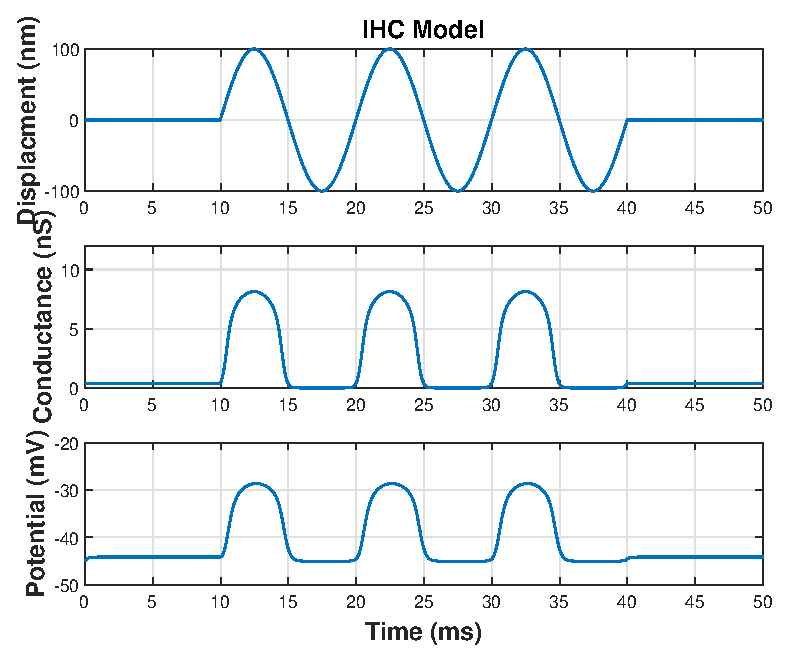
\includegraphics[width=.5\linewidth]{ue3/100Hz_100nm.eps} % oder statt scale auch [width=0.5\textwidth] für eine feste Größe
  \caption{Reaction of an Inner Hair Cell to an external stimulus with \SI{100}{\nano\meter} peak displacement at \SI{100}{\hertz}}
  \label{fig:signal100}
\end{figure}


\begin{figure}[h] 
  \centering
  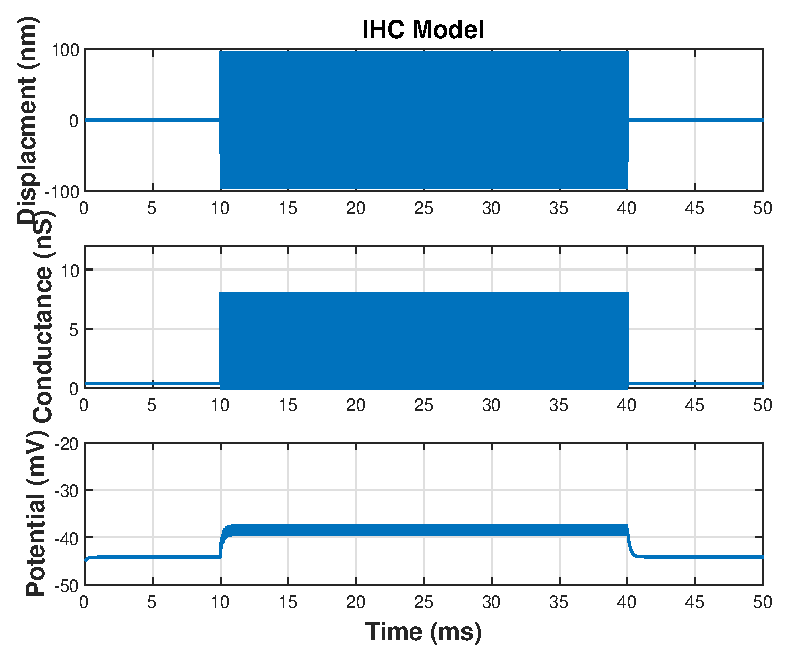
\includegraphics[width=.5\linewidth]{ue3/10kHz_100nm.eps} % oder statt scale auch [width=0.5\textwidth] für eine feste Größe
  \caption{Reaction of an Inner Hair Cell to an external stimulus with \SI{100}{\nano\meter} peak displacement at \SI{10}{\kilo\hertz}}
  \label{fig:signal10k}
\end{figure}

\clearpage
\subsubsection{}
Second, we evaluated the non-linearity of the system by looking at the amplitude spectra of input (Fig. \ref{fig:signal:U_in}) and output (Fig. \ref{fig:signal:U_ihc})  as well as at the actuation conductivity (Fig. \ref{fig:signal:ga}). At a frequency-confined displacement at the input, we got several harmonics in the output frequency at the same frequency. Hereby, the rad dash indicates the \SI{200}{\hertz} of our initial actuation. In contrast to a LTI-system, the fluid interacts nonlinearly after the Navier-Stokes-Equation with the stereocilia.

\begin{figure}[h] 
  \centering
  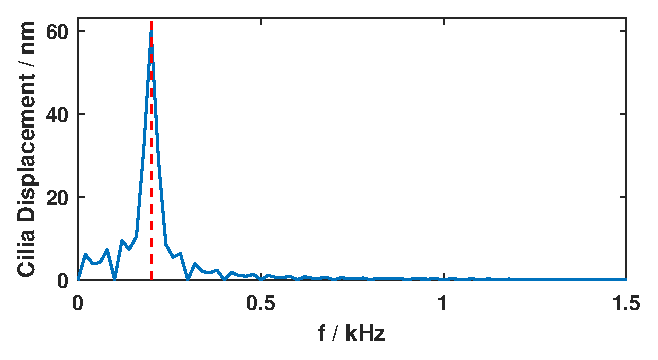
\includegraphics[width=.5\linewidth]{ue3/U_in_200Hz_100nm.eps} % oder statt scale auch [width=0.5\textwidth] für eine feste Größe
  \caption{Spectrum of the input wave. A sinusoidal wave, which displaces the stereocilia of the IHC and triggers its activation.}
  \label{fig:signal:U_in}
\end{figure}
\begin{figure}[h] 
  \centering
  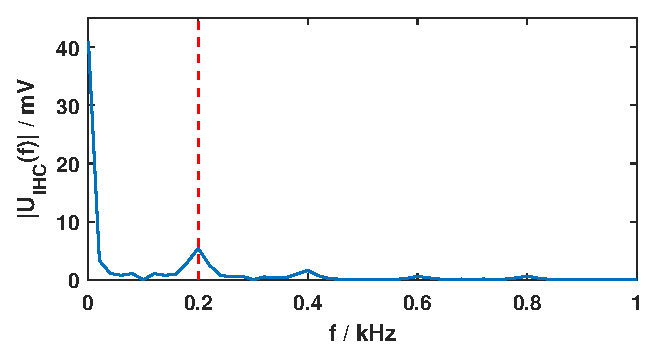
\includegraphics[width=.5\linewidth]{ue3/U_IHC_200Hz_100nm.eps} % oder statt scale auch [width=0.5\textwidth] für eine feste Größe
  \caption{Output voltage of the in Fig. \ref{fig:signal:U_in} excited inner hair cell.}
  \label{fig:signal:U_ihc}
\end{figure}
\begin{figure}[h] 
  \centering
  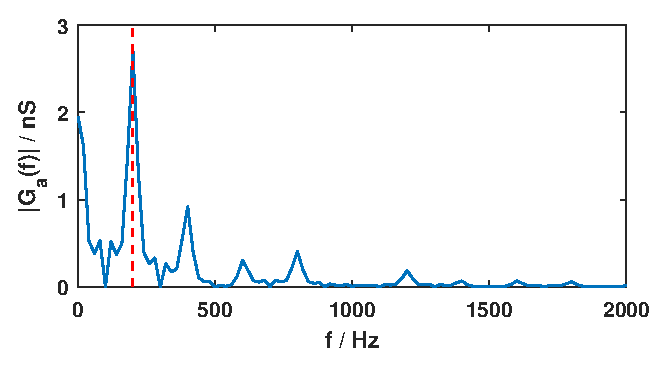
\includegraphics[width=.5\linewidth]{ue3/G_a_200Hz_100nm.eps} % oder statt scale auch [width=0.5\textwidth] für eine feste Größe
  \caption{Receptor conductance for a displacement of \SI{100}{\nano\meter} in its peak at \SI{200}{\hertz}}
  \label{fig:signal:ga}
\end{figure}





\clearpage
\subsubsection{}
As developed in the equations below, we can show, that the system is divergent at a displacement of \SI{100}{\nano\meter} with \SI{200}{\hertz} below a sampling rate of \SI{2789}{\hertz}. The divergence is shown in figure \ref{fig:signal:200Hz_100nm_divergent}, where figure \ref{fig:signal:200Hz_100nm} acts as the convergent reference. 

\begin{figure}[h] 
  \centering
  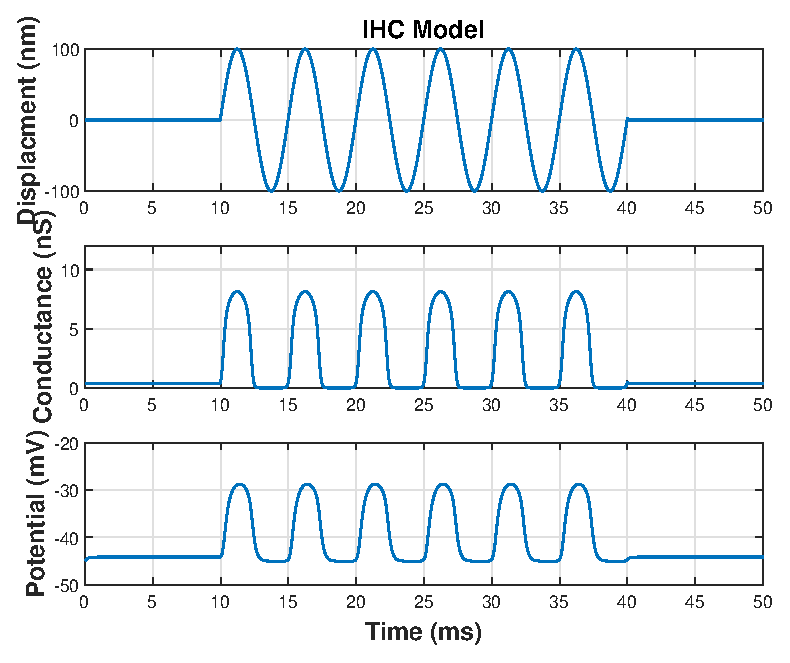
\includegraphics[width=.5\linewidth]{ue3/200Hz_100nm.eps} % oder statt scale auch [width=0.5\textwidth] für eine feste Größe
  \caption{Reaction of an Inner Hair Cell to an external stimulus with \SI{100}{\nano\meter} peak displacement at \SI{200}{\hertz}}
  \label{fig:signal:200Hz_100nm}
\end{figure}

\begin{figure}[h] 
  \centering
  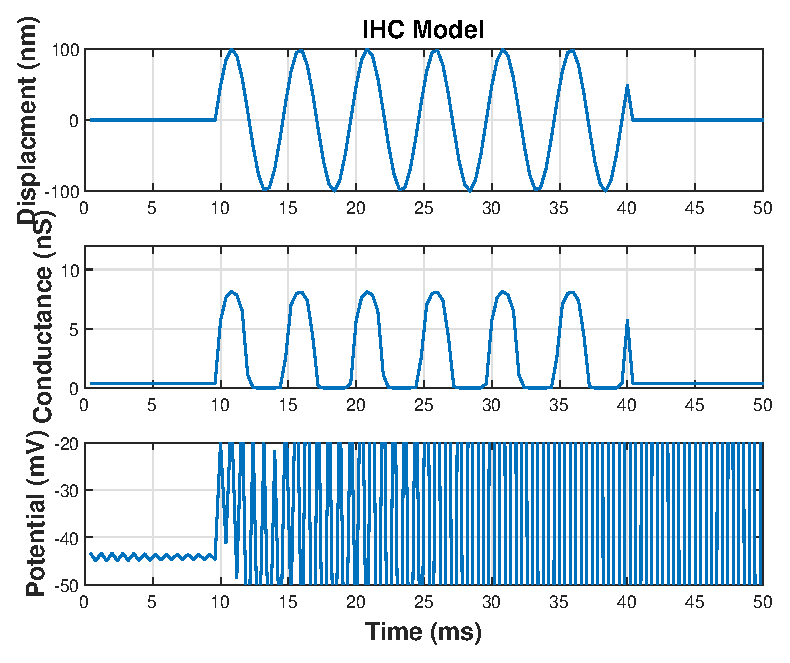
\includegraphics[width=.5\linewidth]{ue3/200Hz_100nm_non_convergent.eps} % oder statt scale auch [width=0.5\textwidth] für eine feste Größe
  \caption{Divergent model driven with the same parameters of \ref{fig:signal:200Hz_100nm}, but at a sample rate of = 2500.}
  \label{fig:signal:200Hz_100nm_divergent}
\end{figure}


The limit was computed by concatenating the three given equations (1), (2) and (3) into the differential equation (Eq. (4)). We substitued for simplification purposes (5) and discretized the continuous differential equation by Euler's Explicit Method (Eqs. 6-8). From there, we conducted a limit of the sequence where the discretized steps tended to infinity. We argument with the geometric series (10), that the term with the highest order had to be smaller than one to let the system converge (Eqs. 9:12). Resolving the inequality concludes to the solution in equation 15. 

An evalation of the dependent parameters led to the insight that the maximum of the stereocilia displacment $x_st$ provides the upper boundary for the step size and therefore the lower boundary for the sampling rate. With the given parameters from above, we can calculate a minimal sampling frequency of \SI{2789}{\hertz}. 


\begin{align}
    \label{eq:model:g_a} g_a(t)\ &=\ \frac{G_{max}}{\left[1 +     exp(\frac{x_0-x{st}(t)}{S_{x0}})\right]\cdot\left[1 +     exp(\frac{x_0-x{st}(t)}{S_{x0}})\right]}\\ 
     \label{eq:model:ir}i_{rez}(t)\ &=\ (EP-u_{IHC}(t))\cdot g_a(t)\\
     \label{eq:model:ib}i_b(t)\ &=\ (V_0 - u_{IHC}(t))\cdot G_b\\
     \label{eq:model:u_ihc}\frac{d}{dt} u_{IHC}(t) &= \frac{i_{rez}(t)\ +\ i_b(t)}{C_m}
\end{align}

\begin{align}
    \frac{d}{dt} u_{IHC}(t) &=  \underbrace{\left(\frac{- g_a - G_b}{C_m}\right)}_{\text{$\mathit{A}$}} \ \cdot\ u_t +\ \underbrace{\frac{EP\cdot g_a + V_0\cdot G_b}{C_m}}_{\text{$\mathit{B}$}} \\
     \frac{d}{dt} u_{IHC}(t) &\approx \frac{\Delta u}{\Delta t} = \frac{u_{t+1}-u_t}{\Delta t}\\
    u_{t+1} &=  \left(1+\mathit{A} \Delta t \right)\ \cdot\ u_t +\ \mathit{B} \Delta t\\
    u_n &= \left(1+\mathit{A} \Delta t \right)^n\ \cdot\ u_0 +\ \mathit{B} \Delta t\ \cdot\ \sum_{i=0}^{n-1}{\left(1+\mathit{A} \Delta t \right)^i}\\
    \lim\limits_{n \to \infty}&\ {\underbrace{\left(1+\mathit{A} \Delta t \right)}_{\text{$\xrightarrow{\text{!}}|1+\mathit{A}\Delta t|<1$}}}^n \ \cdot\ u_0 +\ \mathit{B} \Delta t\ \cdot\ \underbrace{\sum_{i=0}^{n-1}{\left(1+\mathit{A} \Delta t \right)^i}}_{\text{$\xrightarrow{n\xrightarrow{}\infty}geom. Series$}}\\
    \sum_{k=0}^{\infty}{a_0\cdot q^k} &= \frac{a_0}{1-q},\ |q|<1\\
    |1+\mathit{A}\Delta t|\ &< 1\  \Rightarrow \ A \overset{\text{!}}{\leq} 0\\
    |A| &= -\frac{- g_a - G_b}{C_m} \geq 0\\
    1-\frac{ g_a+ G_b}{C_m}\cdot\Delta t &> -1\\
    \frac{ g_a + G_b}{C_m} \cdot\Delta t &< 2\\
    \Delta t &< \frac{2C_m}{g_a+G_b}\\\
    min(g_a(t)) \Rightarrow max(x_{st}) &=\SI{100}{\nano \meter} \Rightarrow min(g_a(t)) = \SI{8.14}{\nano \siemens}\\
    \Delta t &< \frac{2\ \cdot\ \SI{12}{\pico \farad}}{\SI{8.14}{\nano \siemens}\ \cdot\ \SI{58.8}{\nano \siemens}} =  \SI{359}{\micro \second}\\
    \Rightarrow \text{Minimum Sampling Rate}\ &=\ \SI{2789}{Hz}
    \end{align}